% % -*- coding:utf-8 -*-
\documentclass[aspectratio=169,10pt]{beamer}
\nonstopmode

\usepackage{appendixnumberbeamer}
\usepackage{graphicx}
\usepackage{url}
\usepackage{cite}
\usepackage{comment}
\usepackage{verbatim}
% color palette
\definecolor{tu01}{HTML}{84B818}
\definecolor{tu02}{HTML}{D18B12}
\definecolor{tu03}{HTML}{1BB5B5}
\definecolor{tu04}{HTML}{F85A3E}
\definecolor{tu05}{HTML}{4B6CFC}
\definecolor{tu06}{HTML}{E3B505}
\definecolor{tu07}{HTML}{AF331D}
\definecolor{tu08}{HTML}{000000}
\definecolor{tu09}{HTML}{AAAAAA}
\definecolor{tu10}{HTML}{444444}
\definecolor{tu11}{HTML}{84B818}

% mixed and light colors
\colorlet{tu01light}{tu01!33}
\colorlet{tu02light}{tu02!33}
\colorlet{tu03light}{tu03!33}
\colorlet{tu04light}{tu04!33}
\colorlet{tu05light}{tu05!33}
\colorlet{tu06light}{tu06!33}
\colorlet{tu07light}{tu07!33}
\colorlet{tu08light}{tu08!33}
\colorlet{tu09light}{tu09!33}
\colorlet{tu10light}{tu10!33}
\colorlet{tu11light}{tu11!33}

\colorlet{tu01midlight}{tu01!50}
\colorlet{tu02midlight}{tu02!50}
\colorlet{tu03midlight}{tu03!50}
\colorlet{tu04midlight}{tu04!50}
\colorlet{tu05midlight}{tu05!50}
\colorlet{tu06midlight}{tu06!50}
\colorlet{tu07midlight}{tu07!50}
\colorlet{tu08midlight}{tu08!50}
\colorlet{tu09midlight}{tu09!50}
\colorlet{tu10midlight}{tu10!50}
\colorlet{tu11midlight}{tu11!50}

\colorlet{tu01dark}{tu01!80!black}
\colorlet{tu02dark}{tu02!80!black}
\colorlet{tu03dark}{tu03!80!black}
\colorlet{tu04dark}{tu04!80!black}
\colorlet{tu05dark}{tu05!80!black}
\colorlet{tu06dark}{tu06!80!black}
\colorlet{tu07dark}{tu07!80!black}
\colorlet{tu08dark}{tu08!80!black}
\colorlet{tu09dark}{tu09!80!black}
\colorlet{tu10dark}{tu10!80!black}
\colorlet{tu11dark}{tu11!80!black}

\colorlet{lightgray}{gray!25}
\colorlet{midlightgray}{gray!50}
\colorlet{anthracite}{black!85}

% aliases
\colorlet{tudo}{tu01}
\colorlet{tuorange}{tu02}
\colorlet{tudolight}{tu01light}

% \usepackage{beamerthememetropolis}
\usetheme[progressbar=frametitle]{metropolis}
\metroset{progressbar=none}
\newcommand{\themename}{\textbf{\textsc{metropolis}}\xspace}


\usepackage{xcolor}
% Remove default navigation symbols
\setbeamertemplate{navigation symbols}{}
\setbeamercolor{background canvas}{bg=white}

% Custom footline with frame numbers on the left and navigation symbols on the right
\setbeamertemplate{footline}{
  \leavevmode%
  \hbox{%
    \begin{beamercolorbox}[wd=.1\paperwidth,ht=2.5ex,dp=1.125ex,leftskip=1em,rightskip=1em]{author in head/foot}%
      \usebeamerfont{footline} \insertframenumber{} / \inserttotalframenumber
    \end{beamercolorbox}%
    \hfill
    \begin{beamercolorbox}[wd=.9\paperwidth,ht=2.5ex,dp=1.125ex,leftskip=1em,rightskip=1em]{author in head/foot}%
      \usebeamerfont{footline} %\insertnavigation{2cm}
    \end{beamercolorbox}%
  }%
  \vskip0pt%
}


\title{Development of an open-source calibration framework\\ for superconducting qubits}
\subtitle{Master degree in Physics}
\author{Elisa Stabilini}
\institute{Università degli Studi di Milano - Department of Physics}
\titlegraphic{\hfill}
\date{July 4th 2025}

\begin{document}

\maketitle

\begin{frame}{Table of contents}
    \setbeamertemplate{section in toc}[sections numbered]
    \setbeamertemplate{subsection in toc}[subsections numbered]  
    \tableofcontents[hideallsubsections]
\end{frame}

\section{Superconducting qubits}

\begin{frame}[t,fragile]{Artificial atoms}
  \begin{columns}
    \begin{column}{0.5\textwidth}
        Qubit: two level system
        Superconducting qubits: use Josephson Junctions to build anharmonic oscillators
        
    \end{column}
  \end{columns}
%Josephson junction
\end{frame}

%
\begin{frame}[t,fragile]{State readout}
  \begin{columns}
    \begin{column}{0.4\textwidth}
      
    \end{column}
    \begin{column}{0.6\textwidth}
      \begin{center}
          \vspace{2mm}
          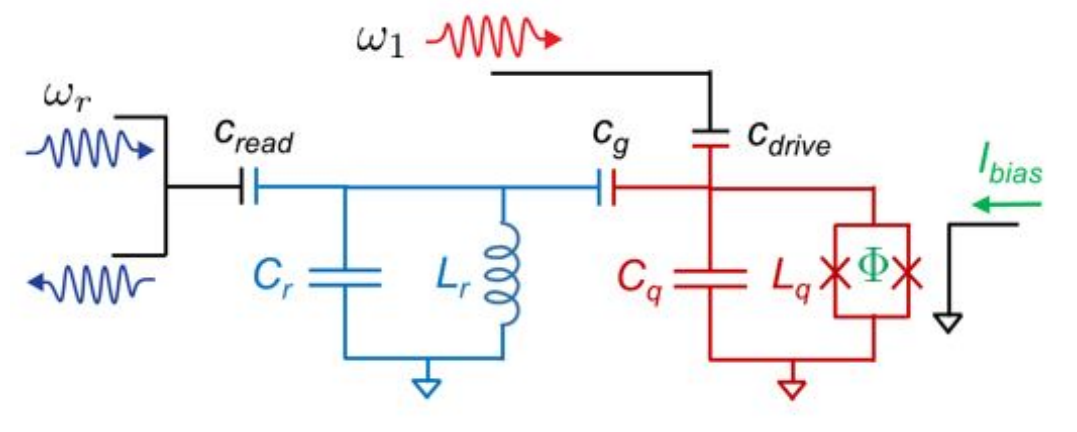
\includegraphics[width=0.85\textwidth]{figures/TransmonCircuit.png}
          \vspace{8mm}
          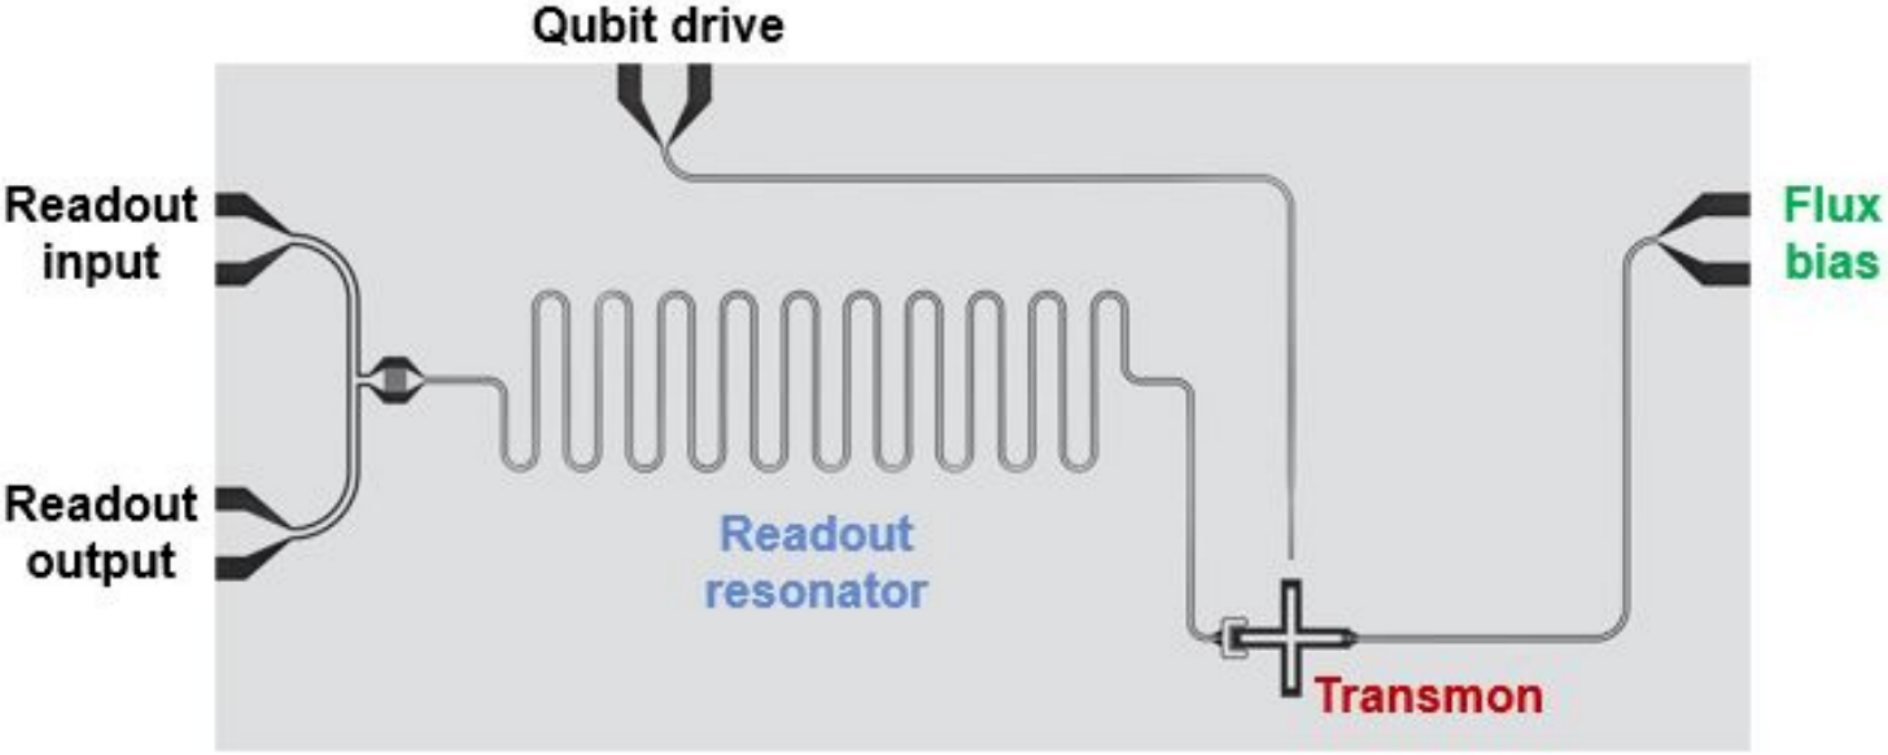
\includegraphics[width=0.85\textwidth]{figures/TransmonBoard.png}
      \end{center}
    \end{column}
  \end{columns}
\end{frame}
%
%\begin{frame}[t,fragile]{Calibration}
%  
%\end{frame}

\begin{frame}[t,fragile]{Qibo framework}
  \begin{center}
      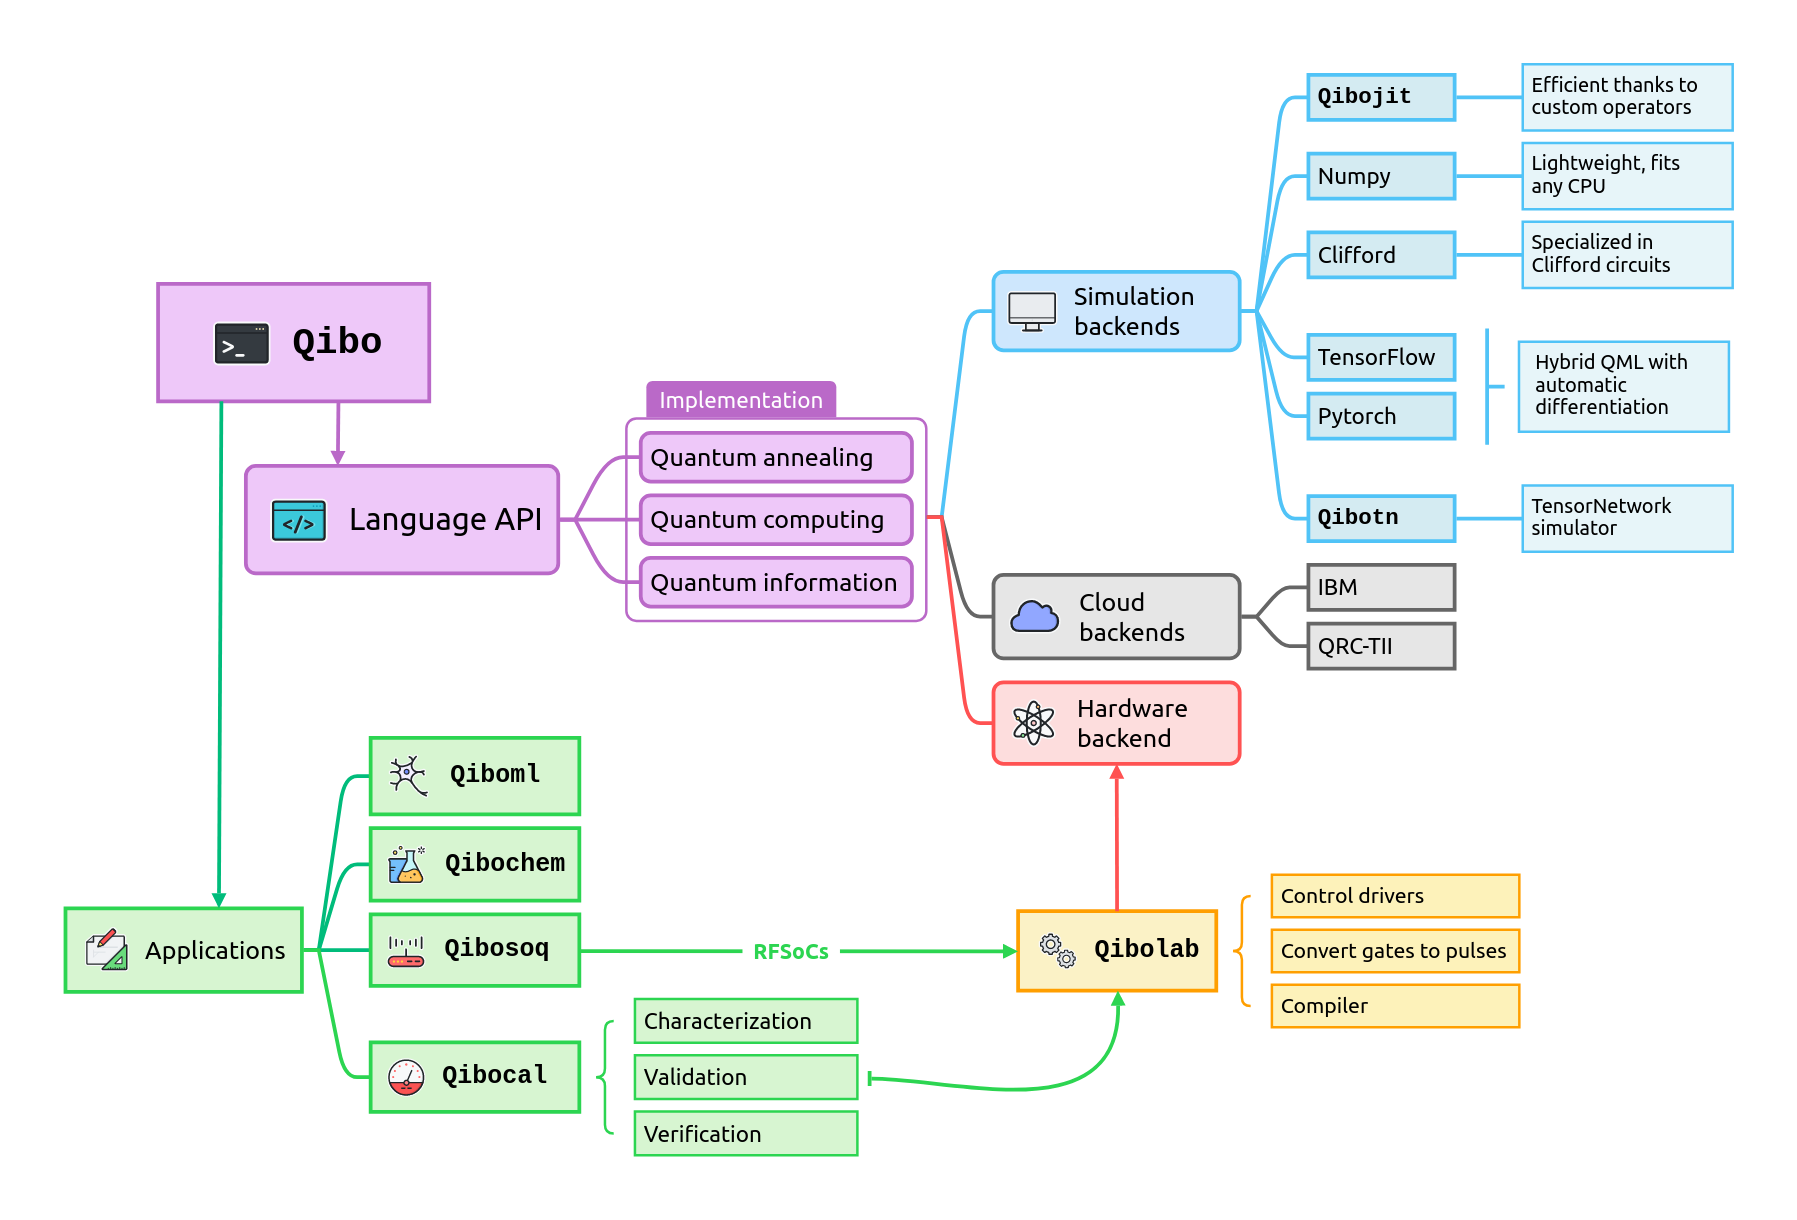
\includegraphics[height=0.80\paperheight]{figures/qibo_ecosystem.png}
  \end{center}
\end{frame}

\section{Avarage Clifford gate fidelity optimization}

%\begin{frame}[t,fragile]{Randomized Benchmarking}
%
%\end{frame}
%
%\begin{frame}[t,fragile]{RB optimization results}
%  
%\end{frame}

\section{Library additions}

\subsection{Native RX90}

%\begin{frame}[t,fragile]{Native RX90 gate}
%  
%\end{frame}

\subsection{Cryoscope}

%\begin{frame}[t,fragile]{Flux pulse reconstruction}
%  
%\end{frame}
%
%\begin{frame}[t,fragile]{Filter determination}
%  
%\end{frame}
%
%\begin{frame}[t,fragile]{Results}
%  
%\end{frame}

\section{Conclusions \& Outlooks}


\begin{frame}[t,standout]
\Large
Questions?
\end{frame}


\begin{frame}{References}
    \nocite{*}
    \bibliographystyle{plain}
    \bibliography{bibliography}
\end{frame}

\begin{frame}{What is for?}
  \begin{columns}
    \begin{column}{0.5\textwidth}
        \textbf{Simulation of quantum system:} "Nature isn't classical, dammit, and if you want to make a simulation of nature, you'd better make it quantum mechanical, and by golly it's a wonderful problem, because it doesn't look so easy"
        %\href{https://link.springer.com/article/10.1007/BF02650179}{\faBook\,\, Richard Feynman, 1982, Simulating Physics with Computers}
      \end{column}
      \begin{column}{0.5\textwidth}
        \begin{center}
            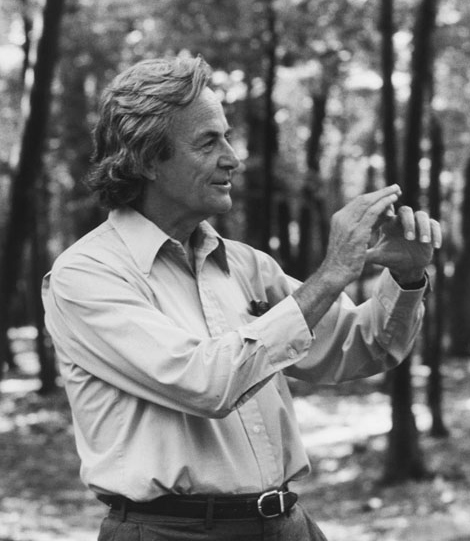
\includegraphics[width=0.8\textwidth]{figures/feynmann.jpg}
        \end{center}
      \end{column}
  \end{columns}
\end{frame}


\begin{frame}{Other quantum computing}
  \begin{enumerate}
    \item Optimization and modeling (finance, traffic, weather...)
    \item Quantum algorithms 
    \item Quantum Machine Learning
  \end{enumerate}
\end{frame}

\begin{frame}{Qubit platforms}
  \begin{center}
      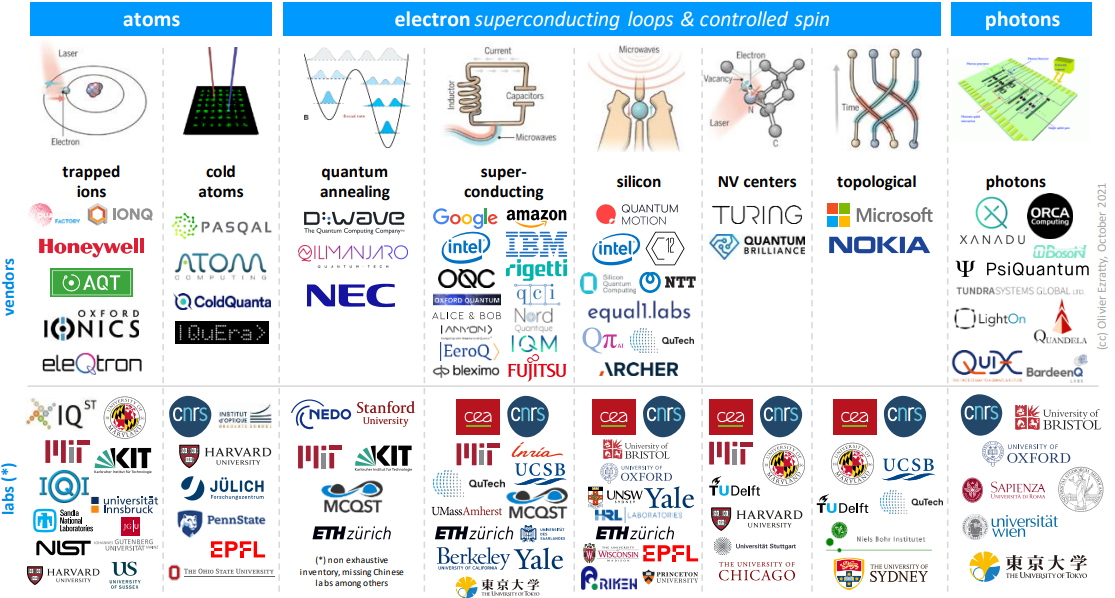
\includegraphics[height=0.8\textheight]{figures/platforms.png}
  \end{center}
\end{frame}

\end{document}
